\documentclass[unknownkeysallowed]{beamer}
\mode<presentation>
{
%  \usetheme{AnnArbor}
%  \usetheme{Dresden}
%  \usetheme{Montpellier}
%  \usetheme{Antibes}
%  \usetheme{Frankfurt}
%  \usetheme{PaloAlto}
%  \usetheme{Bergen}
%  \usetheme{Boadilla}
%  \usetheme{Goettingen}
%  \usetheme{Pittsburgh}	%!!
%  \usetheme{Berkeley}
%  \usetheme{Hannover}
%  \usetheme{Rochester}		%!!!
%  \usetheme{Berlin}
%  \usetheme{Ilmenau}
%  \usetheme{Singapore}
  \usetheme{Boadilla}		%viel platz
%  \usetheme{JuanLesPins}
%  \usetheme{Szeged}		%!
%  \usetheme{boxes}
%  \usetheme{Luebeck}
%  \usetheme{Warsaw}
%  \usetheme{Copenhagen}
%  \usetheme{Madrid}
%  \usetheme{Darmstadt}
%  \usetheme{Malmoe}
%  \usetheme{default}
%  \usetheme{JuanLesPins}

%  \usetheme{Marburg}


%\usefonttheme{professionalfonts}
%	default | professionalfonts | serif |
%	structurebold | structureitalicserif |
%	structuresmallcapsserif
%\useinnertheme{rounded}
%	circles | default | inmargin |
%	rectangles | rounded

%  \setbeamercovered{transparent}
  % oder auch nicht
\usecolortheme{rose}


\definecolor{uaf yellow}{cmyk}{0,0.16,1,0} % official UAF yellow
\definecolor{light yellow}{cmyk}{0.01,0,0.16,0}
\definecolor{uaf blue}{cmyk}{1,0.66,0,0.02} % official UAF blue
\definecolor{light blue}{cmyk}{0.22,0.11,0,0}
\definecolor{arsc blue}{HTML}{005496}
\definecolor{arsc red}{HTML}{a20a42}
\definecolor{arsc green}{HTML}{009a82}
\definecolor{light gray}{HTML}{777777}

  %navigation aus, klaut nur platz
  \setbeamertemplate{navigation symbols}{}
% Reset title background to default
%\setbeamertemplate{title page}[default]
\setbeamercolor{title}{bg=}
\setbeamercolor{frametitle}{bg=uaf blue, fg=white}
\setbeamercolor{institute}{fg=white}
\setbeamercolor{date}{fg=white}
\setbeamercolor{block}{bg=}
%\setbeamercolor{title}{fg=black}

% Reset block background to default
%\setbeamertemplate{blocks}[default]
%\setbeamercolor{block title}{bg=}
%\setbeamercolor{block body}{bg=}

\beamertemplatenavigationsymbolsempty  
\setbeamertemplate{blocks}[rounded][shadows=false]

\useinnertheme{circles}

}
\usepackage[latin1]{inputenc}
\usepackage{latexsym}
\usepackage{amsfonts}
%\usepackage{natbib}
\usepackage{fancyhdr}
\usepackage{graphicx}
%\usepackage{subfigure}
% oder was auch immer
\usepackage{grffile}
\usepackage{pgf}
\usepackage{tikz}

\usepackage{listings}

\usepackage{times}
\usepackage[T1]{fontenc}
%\usepackage{appendixnumber}
% Oder was auch immer. Zu beachten ist, das Font und Encoding passen
% m�ssen. Falls T1 nicht funktioniert, kann man versuchen, die Zeile
% mit fontenc zu l�schen.

\hypersetup{
    bookmarks=true,         % show bookmarks bar?
    unicode=false,          % non-Latin characters in Acrobat's bookmarks
    pdftoolbar=true,        % show Acrobat's toolbar?
    pdfmenubar=true,        % show Acrobat's menu?
    pdffitwindow=false,     % window fit to page when opened
    pdfstartview={FitH},    % fits the width of the page to the window
    pdftitle={My title},    % title
    pdfauthor={Author},     % author
    pdfsubject={Subject},   % subject of the document
    pdfcreator={Creator},   % creator of the document
    pdfproducer={Producer}, % producer of the document
    pdfkeywords={keyword1} {key2} {key3}, % list of keywords
    pdfnewwindow=true,      % links in new window
    colorlinks=false,       % false: boxed links; true: colored links
    linkcolor=red,          % color of internal links
    citecolor=green,        % color of links to bibliography
    filecolor=magenta,      % color of file links
    urlcolor=cyan           % color of external links
}

\title[PAG]% (optional, nur bei langen Titeln n�tig)
{GEOS 436 / 636\\
Programming and Automation for Geoscientists\\[20pt]
-- Week 09: Unix -- Getting Data --
}

\author[Grapenthin]% (optional, nur bei vielen Autoren)
{Ronni Grapenthin\\
rgrapenthin@alaska.edu\\
Elvey 413B\\
x7682}
% - Namen m�ssen in derselben Reihenfolge wie im Papier erscheinen.
% - Der \inst{?} Befehl sollte nur verwendet werden, wenn die Autoren
%   unterschiedlichen Instituten angeh�ren.

\institute[UAF] % (optional, aber oft n�tig)
{}
% - Der \inst{?} Befehl sollte nur verwendet werden, wenn die Autoren
%   unterschiedlichen Instituten angeh�ren.
% - Keep it simple, niemand interessiert sich f�r die genau Adresse.

% - Namen m�ssen in derselben Reihenfolge wie im Papier erscheinen.
% - Der \inst{?} Befehl sollte nur verwendet werden, wenn die Autoren
%   unterschiedlichen Instituten angeh�ren.

% - Der \inst{?} Befehl sollte nur verwendet werden, wenn die Autoren
%   unterschiedlichen Instituten angeh�ren.
% - Keep it simple, niemand interessiert sich f�r die genau Adresse.

\date[]{}

% - Volle oder abgek�rzter Name sind m�glich.
% - Dieser Eintrag ist nicht f�r das Publikum gedacht (das wei�
%   n�mlich, bei welcher Konferenz es ist), sondern f�r Leute, die diese
%   Folien sp�ter lesen.

%\AtBeginSection[]
%{
%  \begin{frame}<beamer>
%    \frametitle{Outline}
%    \tableofcontents[currentsection,currentsubsection]
%  \end{frame}
%}

% Falls Aufz�hlungen immer schrittweise gezeigt werden sollen, kann
% folgendes Kommando benutzt werden:

%\beamerdefaultoverlayspecification{<+->}

%%switch on to have only frame numbers
\setbeamertemplate{footline}[frame number]

\defbeamertemplate*{title page}{customized}[1][]
{
		\begin{tikzpicture}
			\node[text width=\textwidth,
				fill=gray!70, 
				fill opacity=0.75,
				text opacity=1,
				rounded corners = 10pt,
				inner sep=2pt]{
				\begin{center}	
			  \usebeamerfont{title}{\bf \usebeamercolor[fg]{title} \inserttitle}
			  \par
			  \usebeamerfont{subtitle}\insertsubtitle\par
			  \bigskip
			  \usebeamerfont{author}\insertauthor\par
			  \bigskip
			  \usebeamerfont{institute}\insertinstitute\par
			  \bigskip
			  \usebeamerfont{date}\insertdate\par
			  \end{center}
			  };
	\end{tikzpicture}		  
%	\vspace{0.4cm}\usebeamercolor[fg]{titlegraphic}\inserttitlegraphic 
%	\begin{flushright}
%	\vspace{-1.25cm}\includegraphics[width=2cm]{../moore_logo_transp.png}\vspace{5cm}
%	\end{flushright}
}

\begin{document}

\lstset{numbers=left, numberstyle=\tiny, stepnumber=2, basicstyle=\ttfamily, numbersep=5pt, xleftmargin=10pt}

\setbeamertemplate{background}{\includegraphics[width=\paperwidth]{/home/roon/Pictures/rooftop_initial.jpg}}

	\begin{frame}
	\begin{center}
		\titlepage
	\end{center}
	\end{frame}

\setbeamertemplate{background}{}

\begin{frame}
\frametitle{}
%	\vspace{2cm}
	\begin{center}
	How can you (easily) get data (in an automated fashion)?		
	\end{center}
%	\vspace{4cm}
%	{\tiny {\color{gray}$^{*}$hint: YES!!!!}}
\end{frame}

\begin{frame}
	\frametitle{}
	\begin{center}
	How do computer networks work? \scriptsize{(at a high level)}
	\end{center}
\end{frame}

\begin{frame}
	\frametitle{The Internet (pop culture)}
	Search Google Images for "Internet":

	\begin{center}
		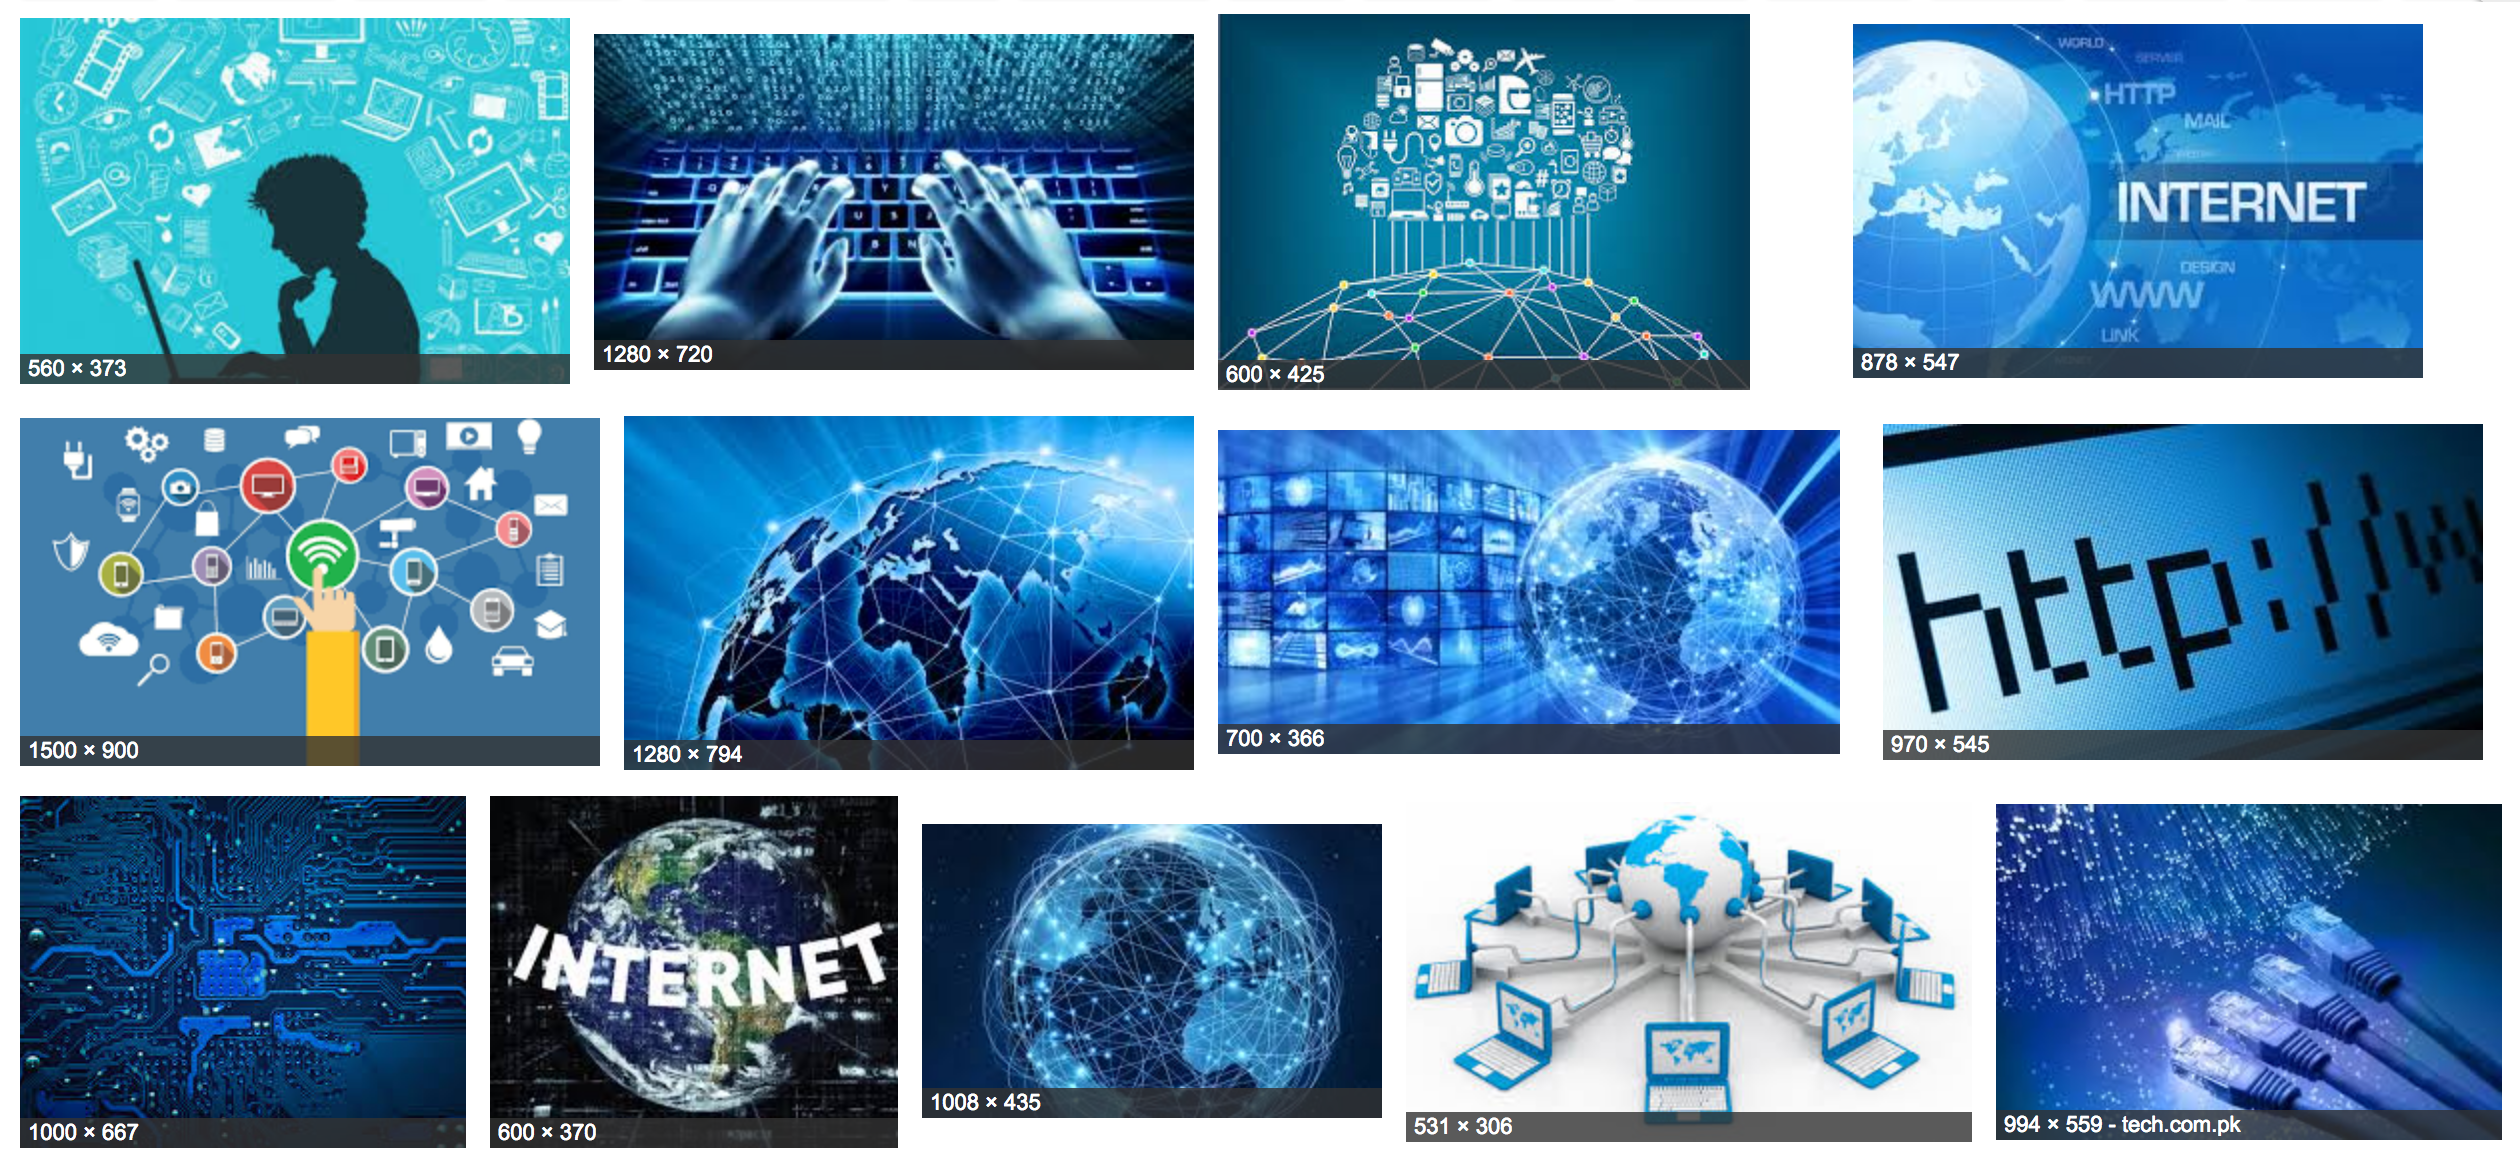
\includegraphics[width=\textwidth]{../figures/internet.png}	
	\end{center}
	\begin{flushleft}
	\tiny{\emph{Google Images}}
	\end{flushleft}	
\end{frame}

\begin{frame}
	\frametitle{Actually (1 client-server pair)}
	\begin{center}
	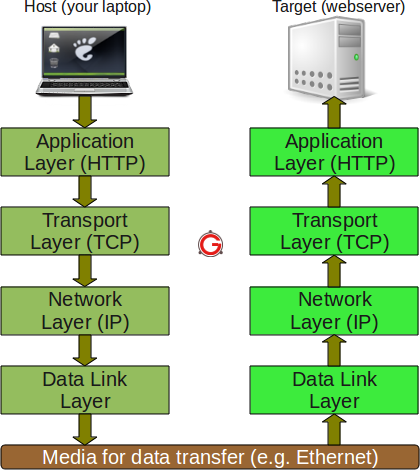
\includegraphics[width=.5\textwidth]{../figures/tcp-ip.png}	
	\end{center}
	\vspace{-0.25cm}
	\begin{flushright}
	\tiny{\emph{Geek Stuff.com}}
	\end{flushright}	
\end{frame} 

\begin{frame}
	\frametitle{The Internet (really)}
	\begin{center}
	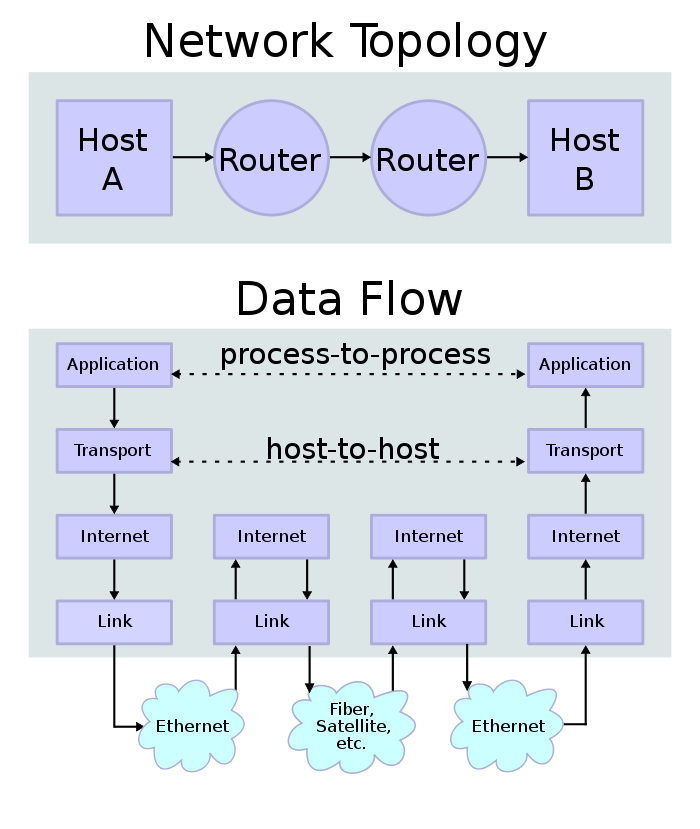
\includegraphics[width=.6\textwidth]{../figures/700px-IP_stack_connections.png}	
	\end{center}
	\vspace{-1.5cm}
	\begin{flushright}
	\tiny{\emph{wikipedia}}
	\end{flushright}	
\end{frame} 

%%%%%%%%%%%%%%%%%
% URLs
%%%%%%%%%%%%%%%%%

\begin{frame}
	\frametitle{URLs}
	\begin{center}
	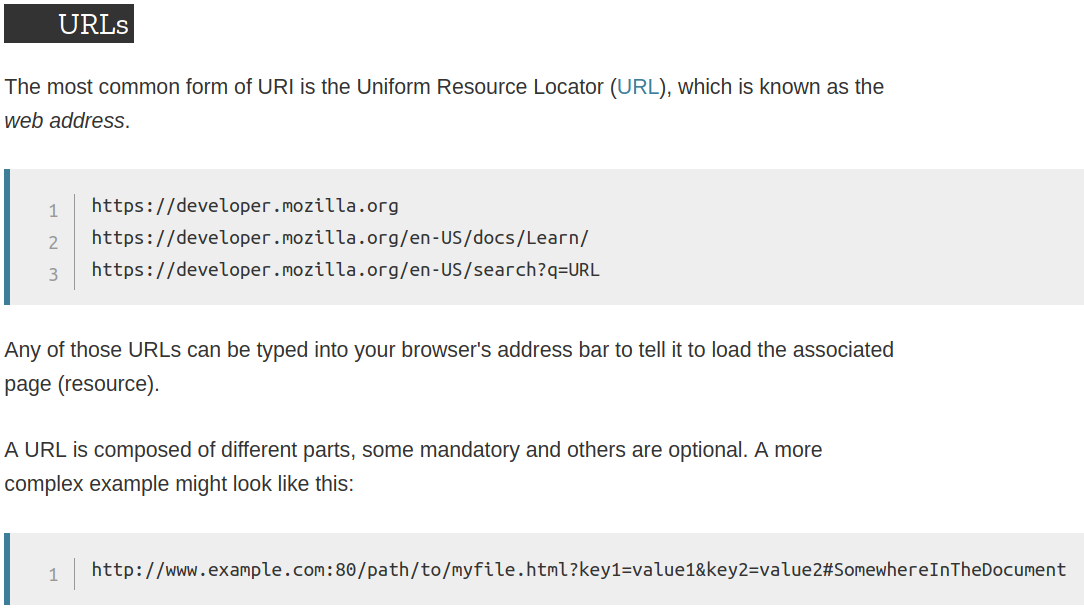
\includegraphics[width=\textwidth]{../figures/url_mozilla_overview.png}	
	\end{center}
	\begin{flushright}
	\tiny{\emph{\href{https://developer.mozilla.org/en-US/docs/Web/HTTP/Basics_of_HTTP/Identifying_resources_on_the_Web}{https://developer.mozilla.org}}}
	\end{flushright}	
\end{frame} 


\begin{frame}
	\frametitle{URLs: Protocol}
	\begin{center}
	
\includegraphics[width=\textwidth]{../figures/url_protocol.png}	
	\end{center}
	\begin{flushright}
	\tiny{\emph{\href{https://developer.mozilla.org/en-US/docs/Web/HTTP/Basics_of_HTTP/Identifying_resources_on_the_Web}{https://developer.mozilla.org}}}
	\end{flushright}	
	usual protocols:
	\begin{itemize}
		\item http, https -- HyperText Transfer Protocol (Secure)
		\item ftp -- FileTransfer Protocol (soon to be obsolete)
		\item mailto: - sometimes comes up to open email client
	\end{itemize}

\end{frame} 

\begin{frame}
	\frametitle{URLs: Domain Name}
	\begin{center}
	
\includegraphics[width=\textwidth]{../figures/url_domain.png}	
	\end{center}
	\begin{flushright}
	\tiny{\emph{\href{https://developer.mozilla.org/en-US/docs/Web/HTTP/Basics_of_HTTP/Identifying_resources_on_the_Web}{https://developer.mozilla.org}}}
	\end{flushright}	
	\begin{itemize}
		\item Can be of varying complexity depending organization
		\item Generally we have top level domains: {\tt .org, .edu, .com, .de}, \dots
		\item You register your domain at a registrar, then you can have various subdomains
		\item e.g.: \url{gi.alaska.edu}
		\item {\tt www.} traditionally (early web days) to distinguish webserver from ftp server ({\tt ftp.}) from mailserver ({\tt smtp., mail.}) etc. and make it known to the public that you're talking about the Internet
	\end{itemize}
\end{frame} 


\begin{frame}
	\frametitle{URLs: Port}
	\begin{center}
	
\includegraphics[width=\textwidth]{../figures/url_port.png}	
	\end{center}
	\begin{flushright}
	\tiny{\emph{\href{https://developer.mozilla.org/en-US/docs/Web/HTTP/Basics_of_HTTP/Identifying_resources_on_the_Web}{https://developer.mozilla.org}}}
	\end{flushright}	
	\begin{itemize}
		\item Indicates which ``entrance'' to the server is to be used.
	\end{itemize}
\end{frame} 


\begin{frame}
	\frametitle{URLs: Path}
	\begin{center}
	
\includegraphics[width=\textwidth]{../figures/url_path.png}	
	\end{center}
	\begin{flushright}
	\tiny{\emph{\href{https://developer.mozilla.org/en-US/docs/Web/HTTP/Basics_of_HTTP/Identifying_resources_on_the_Web}{https://developer.mozilla.org}}}
	\end{flushright}	
	\begin{itemize}
		\item Used to be a path to a physical file on a webserver.
		\item These days there's a lot of abstraction happening
	so it may not reflect actual file structure anymore.
	\end{itemize}
\end{frame} 


\begin{frame}
	\frametitle{URLs: Query / Parameters}
	\begin{center}
	
\includegraphics[width=\textwidth]{../figures/url_parameters.png}	
	\end{center}
	\begin{flushright}
	\tiny{\emph{\href{https://developer.mozilla.org/en-US/docs/Web/HTTP/Basics_of_HTTP/Identifying_resources_on_the_Web}{https://developer.mozilla.org}}}
	\end{flushright}	
	The (for our purposes) very useful part!	
	\begin{itemize}
		\item Key-value pairs that are given to the webserver
		\item Webserver interprets these and responds dynamically to the request
		\item You may be able to exploit this in download scripts
	\end{itemize}
\end{frame} 


\begin{frame}
	\frametitle{URLs: Anchor}
	\begin{center}
	
\includegraphics[width=\textwidth]{../figures/url_anchor.png}	
	\end{center}
	\begin{flushright}
	\tiny{\emph{\href{https://developer.mozilla.org/en-US/docs/Web/HTTP/Basics_of_HTTP/Identifying_resources_on_the_Web}{https://developer.mozilla.org}}}
	\end{flushright}	
	\begin{itemize}
		\item Sort of a bookmark in a document, only used locally (not sent to server)
		\item For an HTML website, the browser scrolls to this spot for you (requires that someone put that anchor in the HTML website)
		\item For audio / video files, browser may go to time it represents
	\end{itemize}
\end{frame} 

%% DATA STORAGE

\begin{frame}
	\frametitle{Data Storage}
	\begin{center}
	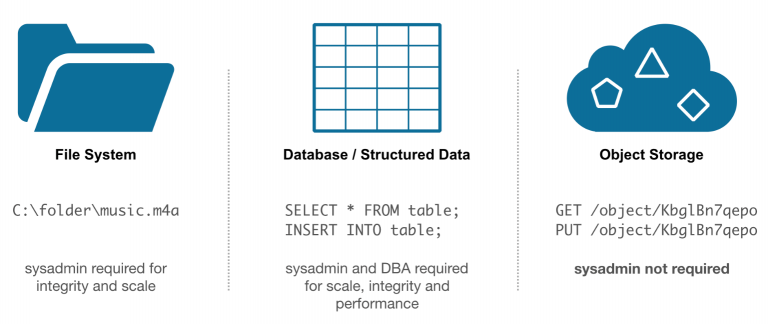
\includegraphics[width=\textwidth]{../figures/data_storage.png}	
	\end{center}
	\begin{flushright}
	\tiny{\emph{ibm}}
	\end{flushright}	
	\begin{itemize}
		\item files: photo, document, ...
		\item database: subset records of interest
		\item object storage: the cloud (appears as file but isn't)
	\end{itemize}
\end{frame} 

\begin{frame}
	\frametitle{A very short list of public data archives }
	\begin{itemize}
		\item IRIS: Seismic / infrasound data - \url{https://ds.iris.edu/ds/nodes/dmc/}
		\item UNAVCO: geodetic data (GNSS mainly, some SAR) - \url{ftp://data-out.unavco.org/pub/products/}
		\item ASF: SAR data - \url{https://search.asf.alaska.edu/}
		\item Waterdata USGS - \url{https://waterdata.usgs.gov/}
		\item NASA Global Sulfur Monitoring - \url{https://so2.gsfc.nasa.gov/}
%		\item https://waterdata.usgs.gov/nwis/uv?cb_72019=on&format=rdb&site_no=302416087505501&period=&begin_date=2020-10-12&end_date=2020-10-19
	\end{itemize}
	Some allow for automated downloads, others don't.
\end{frame}

%% DATA ACCESS

\begin{frame}
	\frametitle{Data Access}
	Is it a one-off download? Just do it manually.\\[10pt]
	If you suspect repeated use, invest some time in writing a script:
	\begin{enumerate}
	\item Explore the archive and strucutre: file-based? webservice?
	\item Experiment with various methods of download \& unpacking (see later)
	\item Generalize for your use case to enable quick downloads in the future (command line arguments for your script).
	\end{enumerate}
\end{frame} 

%\begin{frame}
%	\frametitle{Webservices}
%	\begin{center}
%	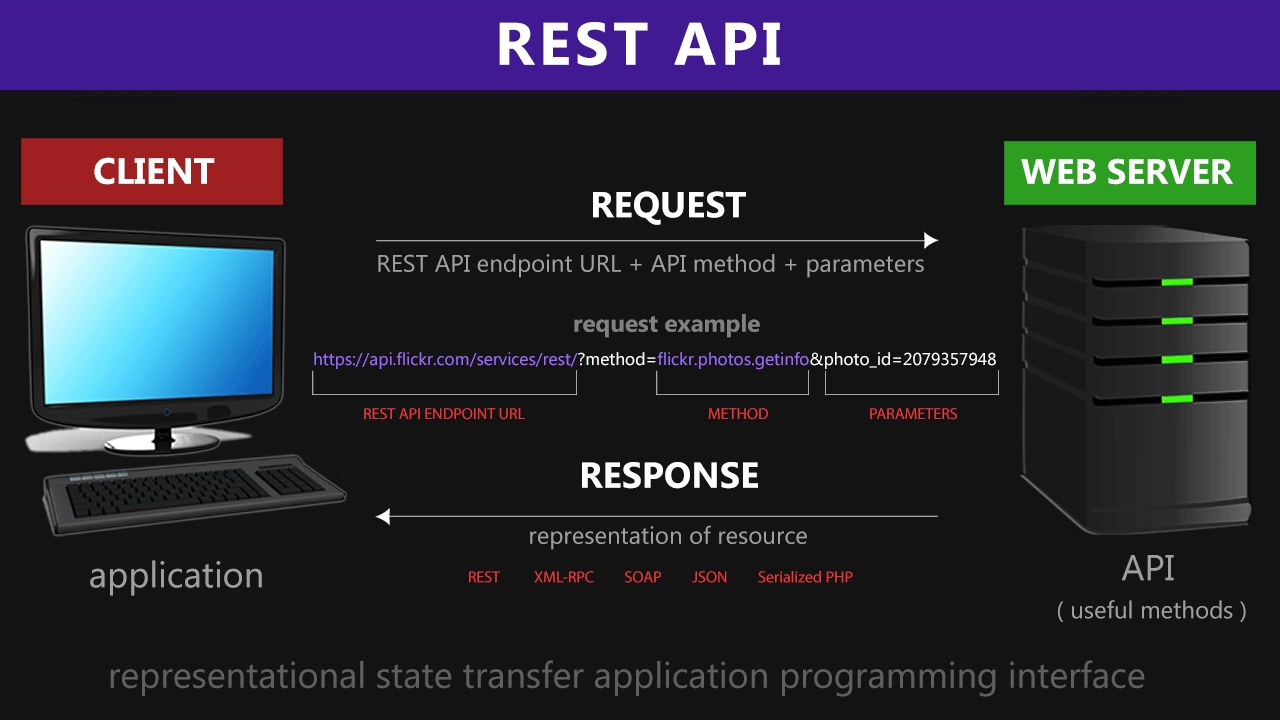
\includegraphics[width=\textwidth]{../figures/REST_API.jpg}	
%	\end{center}
%	\begin{flushright}
%	\tiny{\emph{\url{https://www.youtube.com/watch?v=LooL6_chvN4}}}
%	\end{flushright}	
%\end{frame} 

\begin{frame}
	\frametitle{Working on a remote machine: {\tt ssh}}
	\begin{center}
	
\includegraphics[width=.6\textwidth]{../figures/ssh.jpg}	
	\end{center}
	\begin{flushright}
	\tiny{\emph{errorhat.com}}
	\end{flushright}	
	\begin{center}
	{\tt \$> ssh -XY user@server.edu}
	\end{center}
	\begin{itemize}
		\item {\tt X,Y} options enable X11 (graphics) forwarding (view windows rendered on remote machine)
		\item {\tt X} is more secure, sometimes has issues
		\item {\tt Y} is a little less secure.
		\item use {\tt exit} to close on remote machine 
	\end{itemize}
\end{frame}

\begin{frame}
	\frametitle{Working on a remote machine: {\tt ssh}}
	Example: 
	\begin{center}
	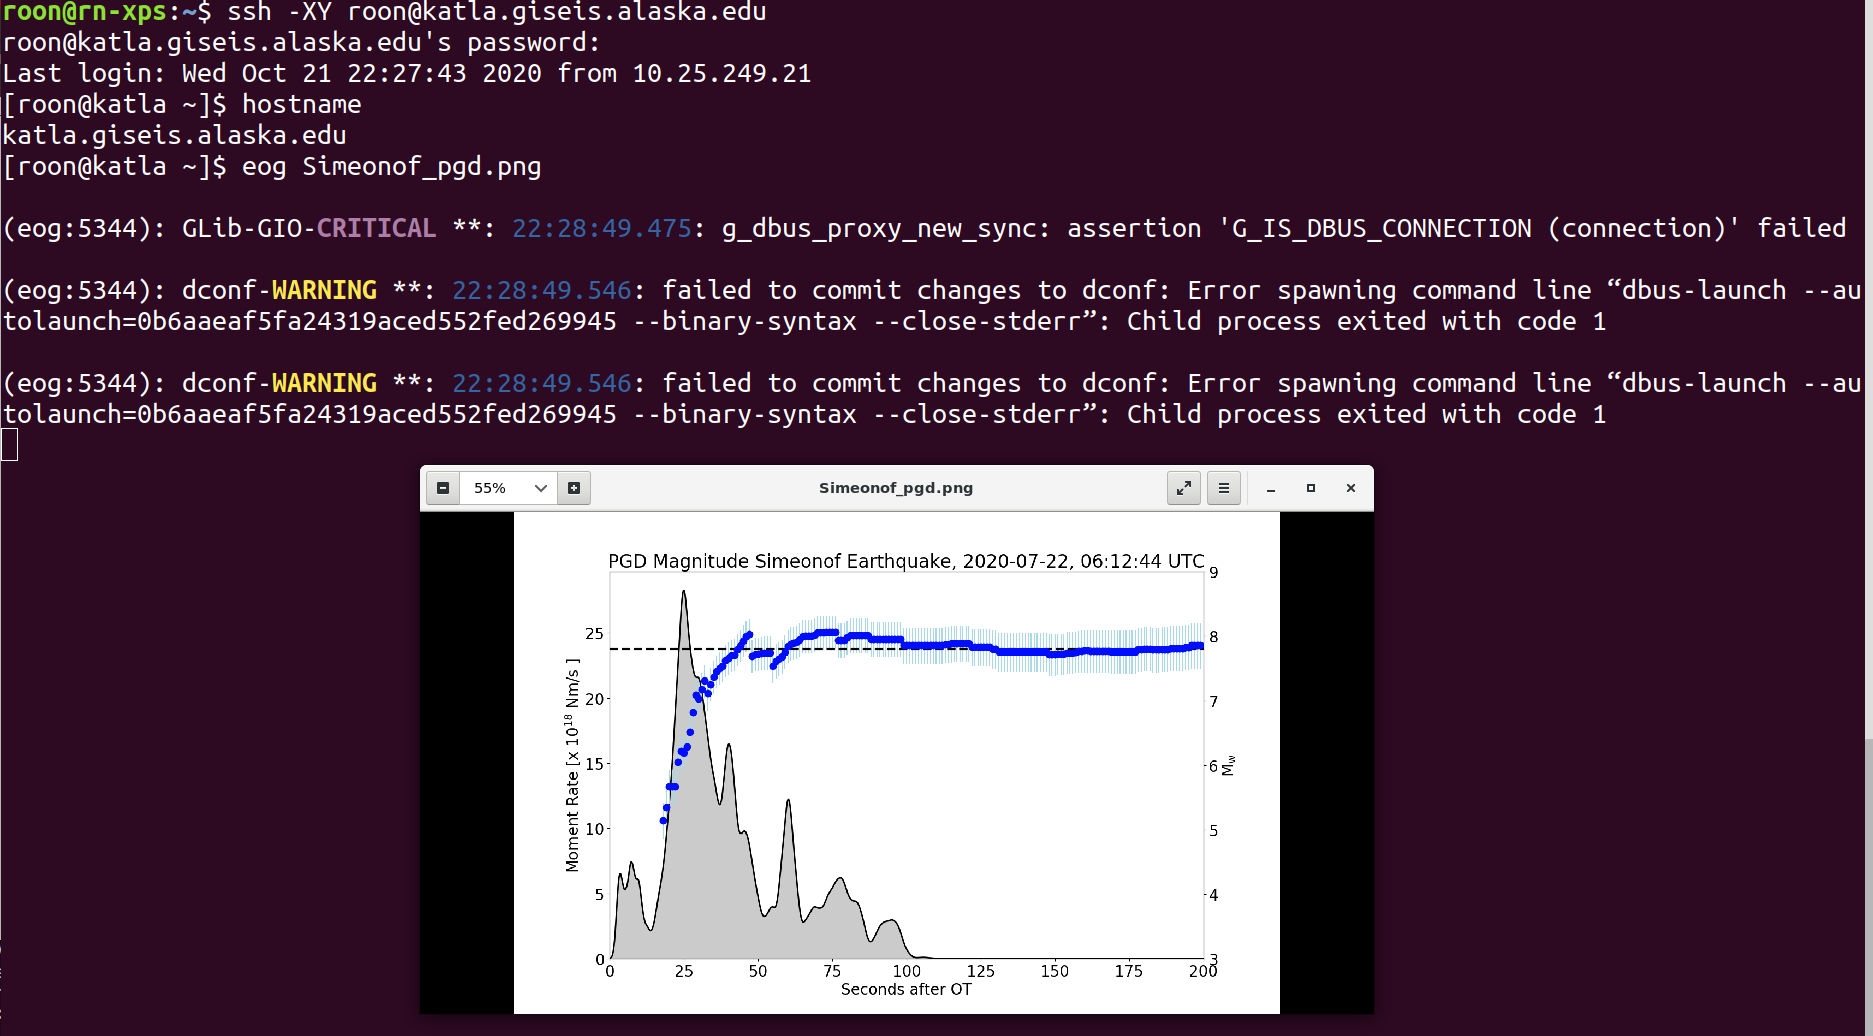
\includegraphics[width=\textwidth]{../figures/ssh_example.png}	
	\end{center}
\end{frame}

\begin{frame}
	\frametitle{Getting Data from Strangers: {\tt wget, curl}}
	Once data access is sorted, you may need to download at the command line:
	\begin{itemize}
		\item {\tt wget}
			\begin{itemize}
				\item recursive downloads (entire directories)
				\item HTTP(s), FTP only
				\item default: download to a file
			\end{itemize}
		\item {\tt curl}
			\begin{itemize}
				\item single URLs only, more protocols, download and upload
				\item preinstalled on MacOS, Windows 10.
				\item default: download to stdout, use {\tt -o} to specify output file
			\end{itemize}
	\end{itemize}

	For most of your needs they are the same and {\tt wget} will get the job done quickly.

\end{frame}

\begin{frame}
	\frametitle{Getting Data from Strangers: {\tt wget}}
	\begin{center}
	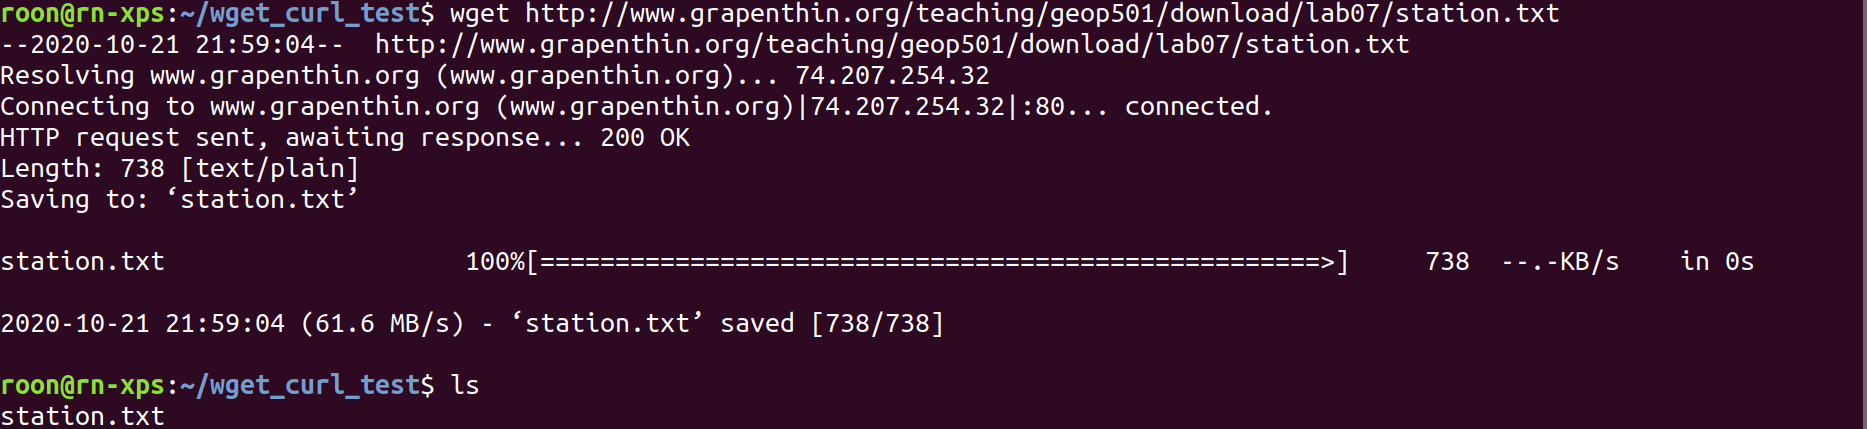
\includegraphics[width=\textwidth]{../figures/wget.png}	
	\end{center}
\end{frame}

\begin{frame}
	\frametitle{Getting Data from Strangers: {\tt curl} 1}
	\begin{center}
	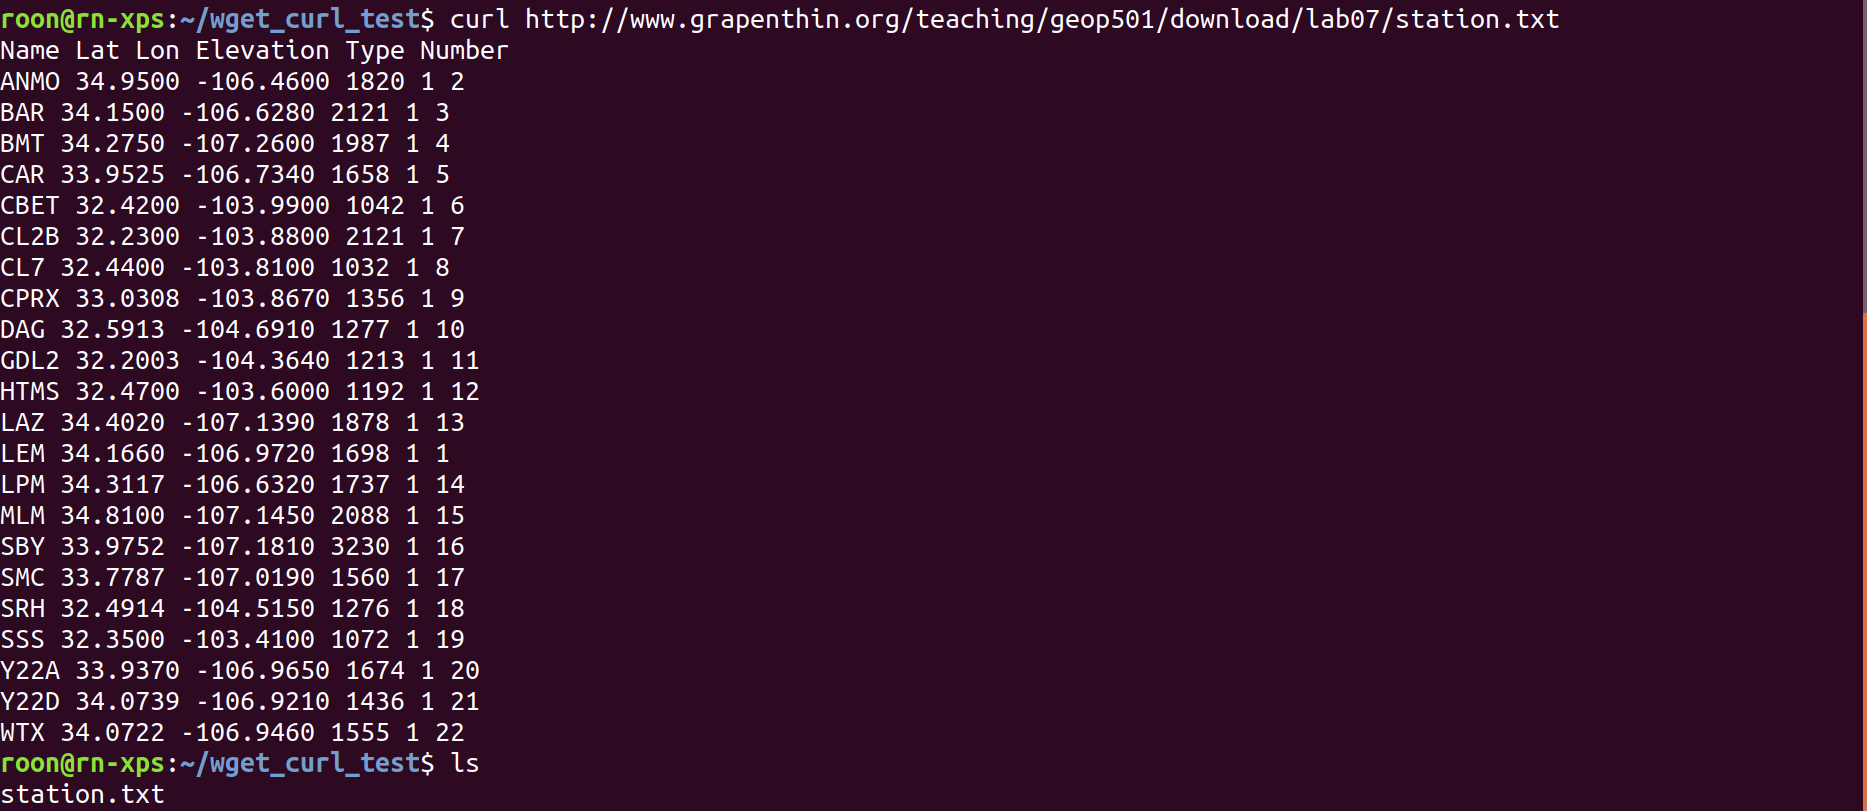
\includegraphics[width=\textwidth]{../figures/curl_1.png}	
	\end{center}
\end{frame}

\begin{frame}
	\frametitle{Getting Data from Strangers: {\tt curl} 2}
	\begin{center}
	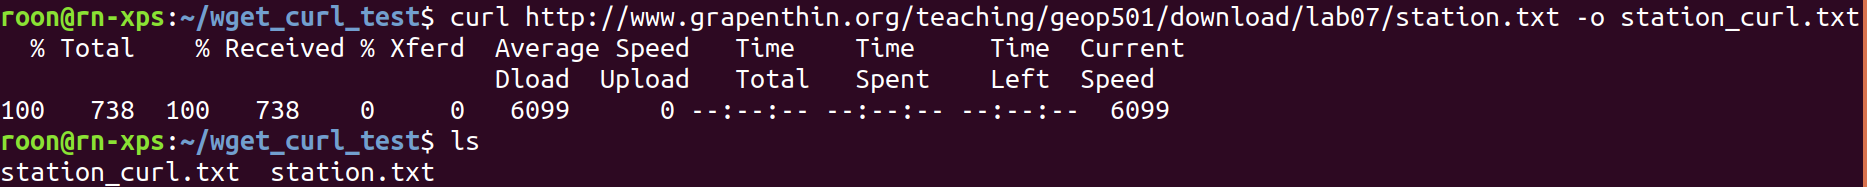
\includegraphics[width=\textwidth]{../figures/curl_2.png}	
	\end{center}
\end{frame}


\begin{frame}
	\frametitle{Transferring Data between (your) machines: {\tt scp}}
	\begin{itemize}
		\item Some work happens on remote machines
		\item Need to get some data / configuration files from local machine there
		\item You may need to retrieve your results from there to local machine
		\item Or transfer from one remote machine to another remote machine
	\end{itemize}
	\begin{center}
	{\tt \$> scp OPTIONS SOURCE(s) TARGET}\\
	{\tt \$> scp [[u1@]host1:]file1 ... [[u2@]host2:]file2}\\
	\end{center}

\end{frame}

\begin{frame}
	\frametitle{Transferring Data between (your) machines: scp}
	\begin{center}
	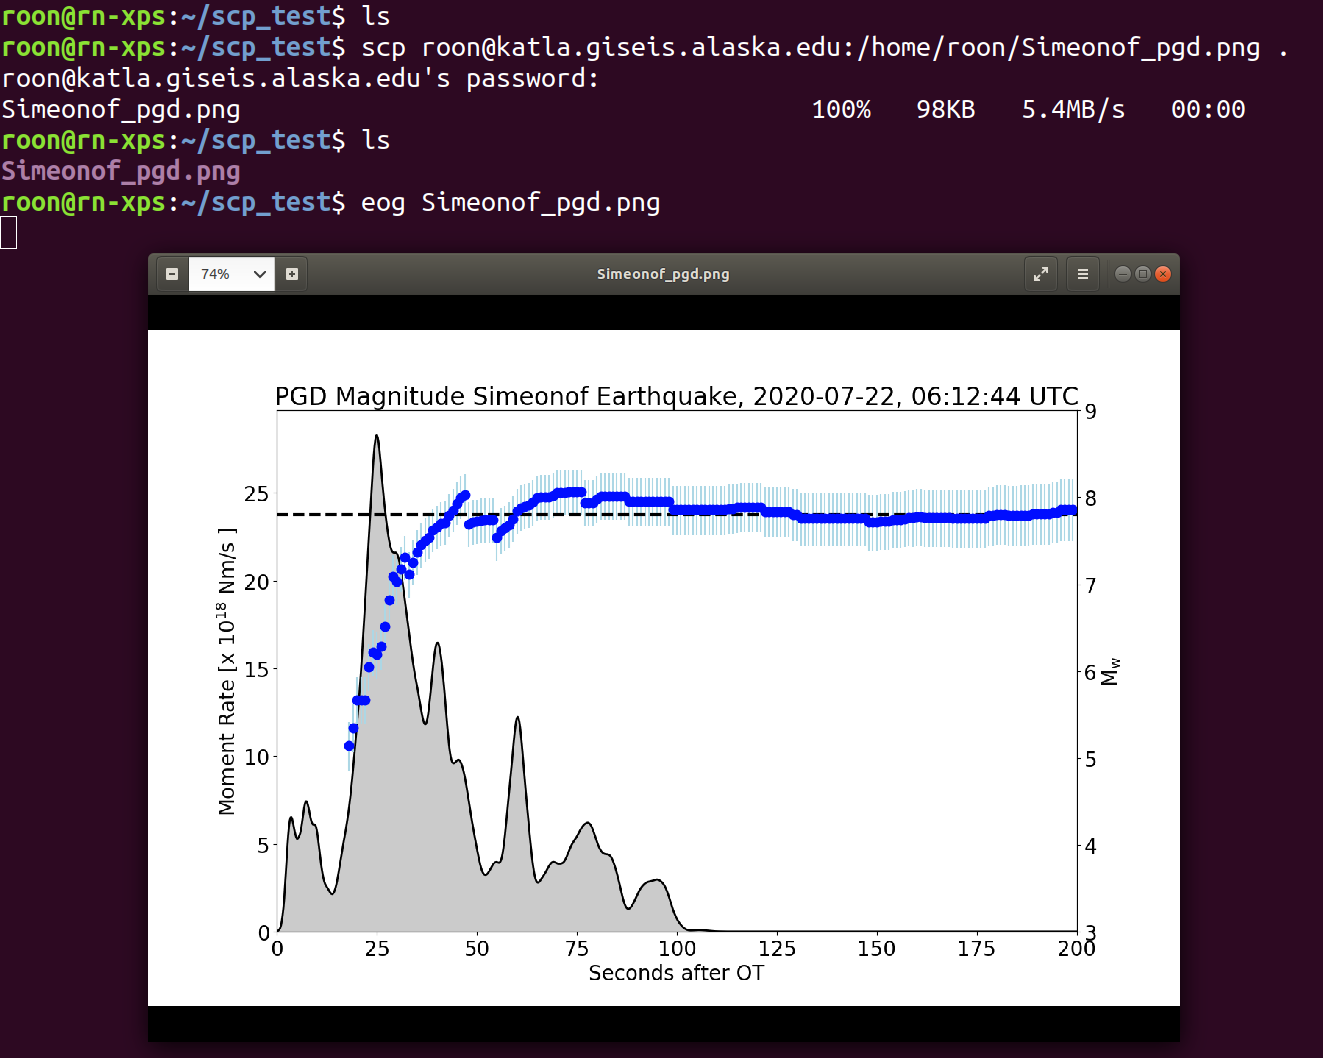
\includegraphics[width=.8\textwidth]{../figures/scp.png}	
	\end{center}

\end{frame}
\begin{frame}
	\frametitle{Transferring Data between (your) machines: scp}
	\begin{center}
	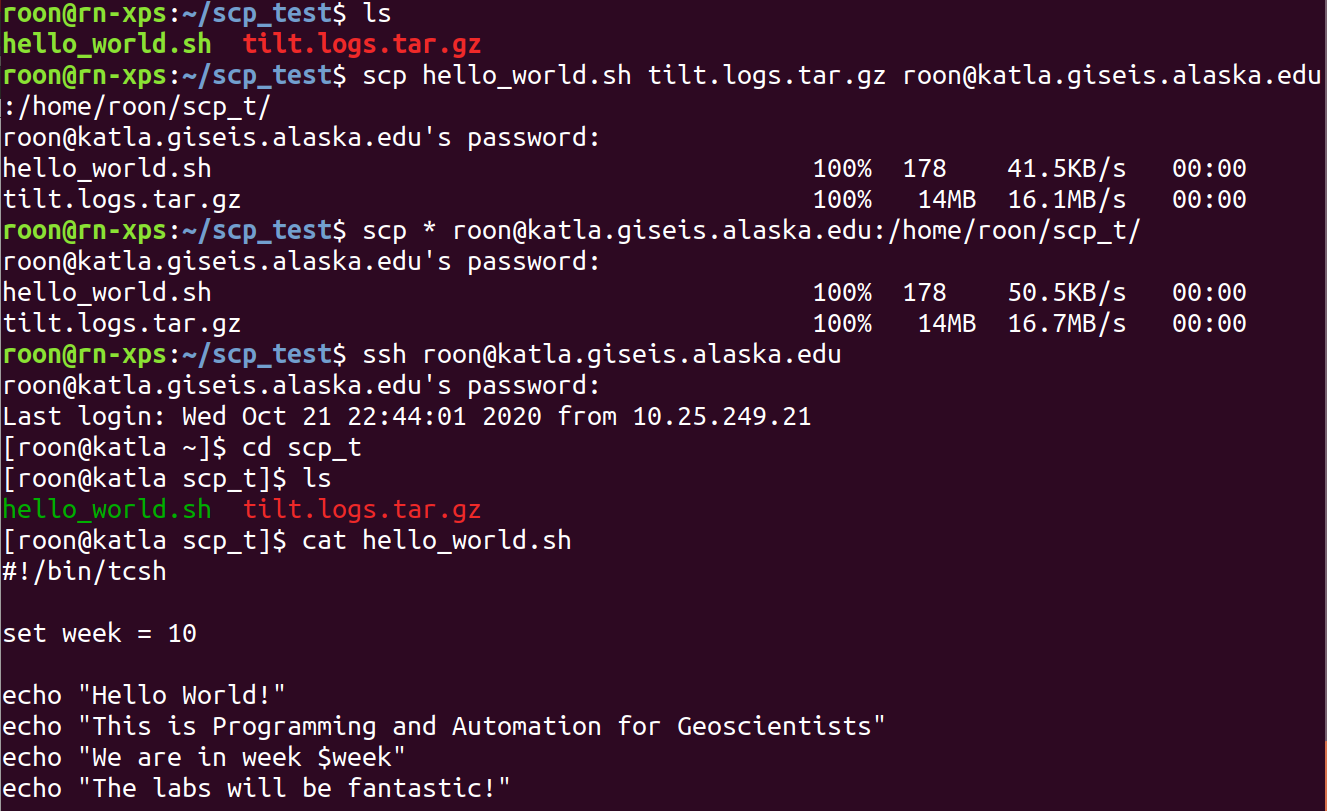
\includegraphics[width=\textwidth]{../figures/scp_example2.png}	
	\end{center}
\end{frame}

%%UNPACKING

\begin{frame}
	\frametitle{Unpacking Data}
	\begin{itemize}
		\item Data (in repositories) are often compressed
		\item Some form of archival format: gzip, tar-gzip, zip, etc.
		\item most common tools on command line:
			\begin{itemize}
				\item {\tt \$> gzip file} -- creates {\tt file.gz}
				\item {\tt \$> gunzip file.gz} -- unpacks {\tt file}
				\item {\tt \$> tar cfz archive.tar.gz files/folder} -- tars files/folder into one file which can be gzipped 
				\item {\tt \$> tar xfz archive.tar.gz} -- ungzips and untars the archive
				\item {\tt \$> unzip file.zip} -- unzips the occassional zip file that comes by
			\end{itemize}	
		\item {\tt tar} is convenient to stuff many files / folders into a single file, which then can be gzip compressed.
	\end{itemize}
\end{frame}

\begin{frame}
	\frametitle{(Un)packing Data: {\tt tar, gzip}}
	\begin{center}
	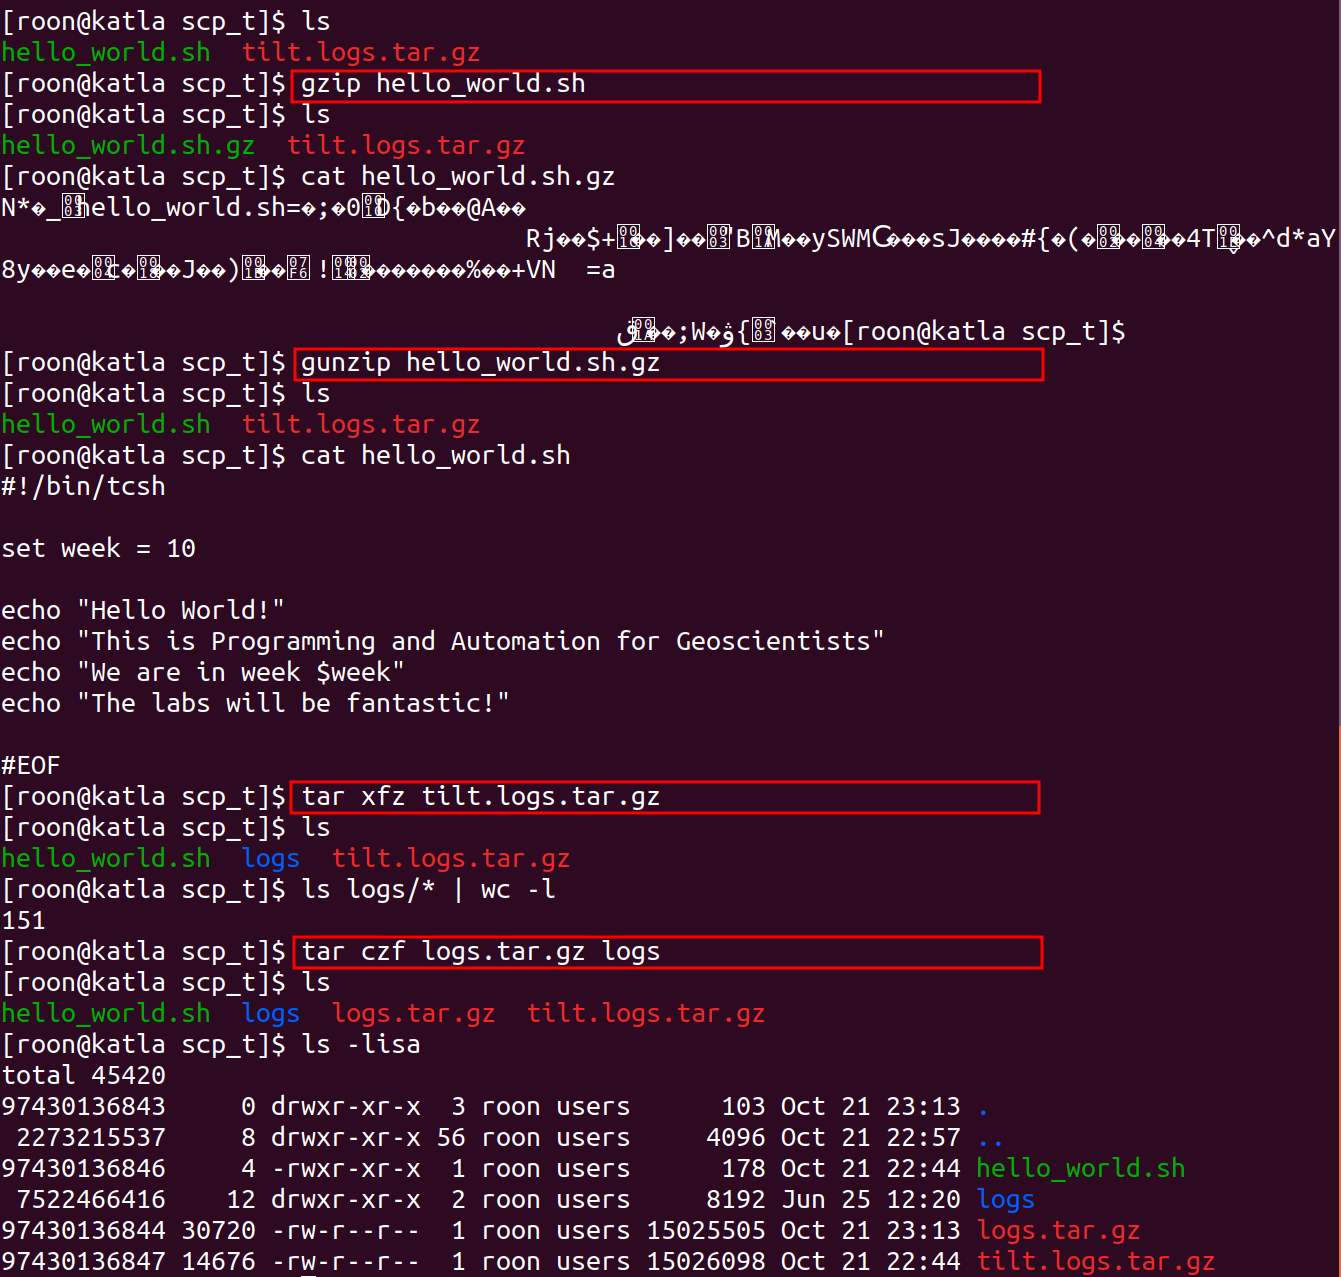
\includegraphics[width=.7\textwidth]{../figures/archiving.png}	
	\end{center}
\end{frame}

\begin{frame}
	\frametitle{Inspecting Data}
	\begin{itemize}
		\item Once you have the data, you need ways to figure out whether they are what you wanted. 
		\item How can you do that quickly without firing up Excel?
		\item {\tt less, head, tail, cat} - we talked about these tools during the last lecture.
	\end{itemize}
\end{frame}

\begin{frame}
	\frametitle{Workflow}
	\begin{columns}[t]
	\column{0.45\textwidth}
		\begin{enumerate}
		\item Manual exploration of archive
		\item Tests with wget/curl/etc. 
		\item Unpacking (tar, gunzip) 
		\item Data inspection (less, more, cat)
		\end{enumerate}
	\column{0.45\textwidth}
		\begin{enumerate}
		\item Think about generalization
		\item Start a shell script with results from manual work
		\item Test on small, diverse subsets of data
		\item Run script automatically, triggered
		\end{enumerate}
	\end{columns}
\end{frame}

\begin{frame}
	\frametitle{Putting it all together}
	\begin{center}
	Let's write a script to download some data from UNAVCO \dots
	\end{center}
\end{frame}


\end{document}
